\section{Combinational VHDL}
\begin{enumerate}
	\item[1)]
	Vi designer systemet som vist på figur \ref{fig:figur1}, med koden \ref{lst:combinationalCode}.
	\begin{figure}[h]
		\centering
		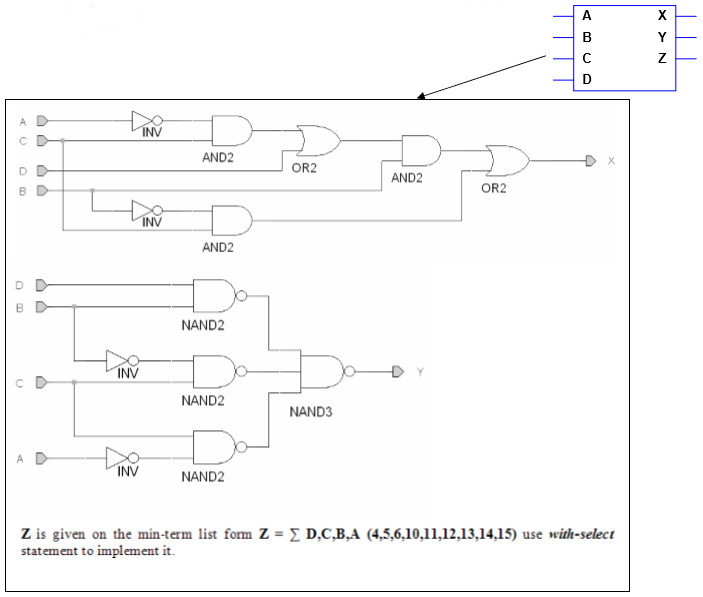
\includegraphics[scale=0.8]{pictures/Oevelse4/figur1.JPG}
		\caption{}
		\label{fig:figur1}
	\end{figure}
	\begin{lstlisting}[caption={Combinational VHDL kode},label={lst:combinationalCode}]
	library ieee;
	use ieee.std_logic_1164.all;
	
	
	entity combinational_VHDL is
	port (a, b, c, d : in std_logic;
	x, y, z : out std_logic);
	end;
	
	architecture dataflow of combinational_VHDL is
	signal tmp : std_logic_vector(3 downto 0);
	begin
	tmp <= (d, c, b, a);
	x <= (((((not a) and c) or d) and b) or ((not b) and c));
	y <= not((not(d and b))and (not((not b)and c)) and (not((not a)and c)));
	with tmp select
	z <= '1' when "0100" |"0101" |"0110" |"1010" |"1011" |"1100" |"1101" |"1110" |"1111",
	'0' when others; 
	
	end dataflow;
	\end{lstlisting}
	
	\item[2)]
	Vi laver nu en functional simulation af koden og får resultatet vist på figur \ref{fig:comVHDLFunSim}. 
		\begin{figure}[h]
			\centering
			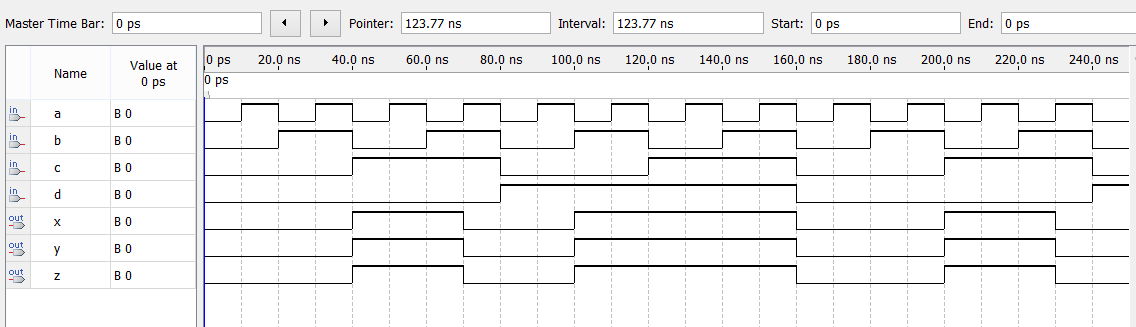
\includegraphics[scale=0.6]{pictures/Oevelse4/combinational_VHDL_Func_sim.jpg}
			\caption{Functional simulation}
			\label{fig:comVHDLFunSim}
		\end{figure}
			\item[3)]
			Med et RTL-view ser vi at systemet er forkortet ned som vist på figur \ref{fig:comVHDLRTL}. 
			\begin{figure}[h]
				\centering
				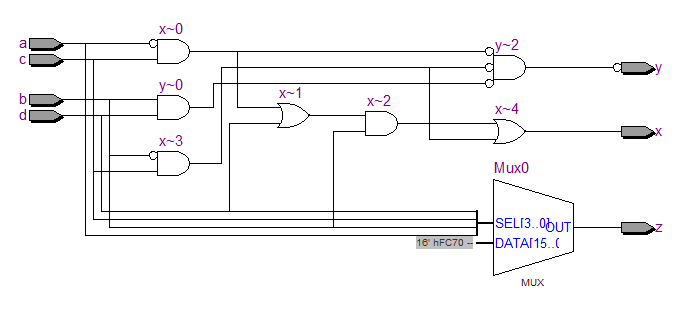
\includegraphics[scale=0.6]{pictures/Oevelse4/combinational_VHDL_RTL.jpg}
				\caption{RTL overview}
				\label{fig:comVHDLRTL}
			\end{figure}
\end{enumerate}